% Designs
\chapter{Design}
\section{Power Calculations}
\begin{table}[!htb]
  \centering
  \renewcommand{\arraystretch}{1.2}
  \begin{tabular}{ |c|c|c|c| }
  \hline
  \textbf{Component}        & \textbf{Voltage}    & \textbf{Current}     & \textbf{Power}   \\
  \hline
  Motors                    & 24 V                & 0.5 A (x4)           & 48 W             \\ \hline
  Motor Drivers             & 5 V                 & 89 mA (x2)           & 890 mW           \\ \hline
  ESP32 Dev Board           & 5 V                 & 120 mA               & 660 mW           \\ \hline
  RA-02                     & 3.3 V               & 100 mA               & 330 mW           \\ \hline
  ATGM332D-5N31             & 3.3 V               & 25 mA                & 82.5 mW          \\ \hline
  MPU-9250                  & 3.3 V               & 3.7 mA               & 12.21 mW         \\ \hline
  \textbf{Total}            &                     &                      & \textbf{49.97 W}         \\ \hline
  \end{tabular}
  \caption{Ground Station Total Power Calculation}
  \label{tab:gs_component_consumption}
\end{table}

\begin{table}[!htb]
  \centering
  \renewcommand{\arraystretch}{1.2}
  \begin{tabular}{ |c|c|c| }
  \hline
  \textbf{Component}        & \textbf{Current}        & \textbf{Power (@ 3V3)}      \\ \hline 
  ATmega328                 & 12 mA                   & 39.6 mW                     \\ \hline 
  RA-02                     & 100 mA                  & 330 mW                      \\ \hline 
  ATGM332D-5N31             & 25 mA                   & 82.5 mW                     \\ \hline
  MAX485                    & 137.3 mA                & 1.0 mW                        \\ \hline
  \textbf{Total}            &                         & \textbf{453.1 mW}         \\ \hline
  \end{tabular}
  \caption{PocketQube Unit Component Power Consumption}
  \label{tab:pqunit_component_consumption}
\end{table}


\clearpage
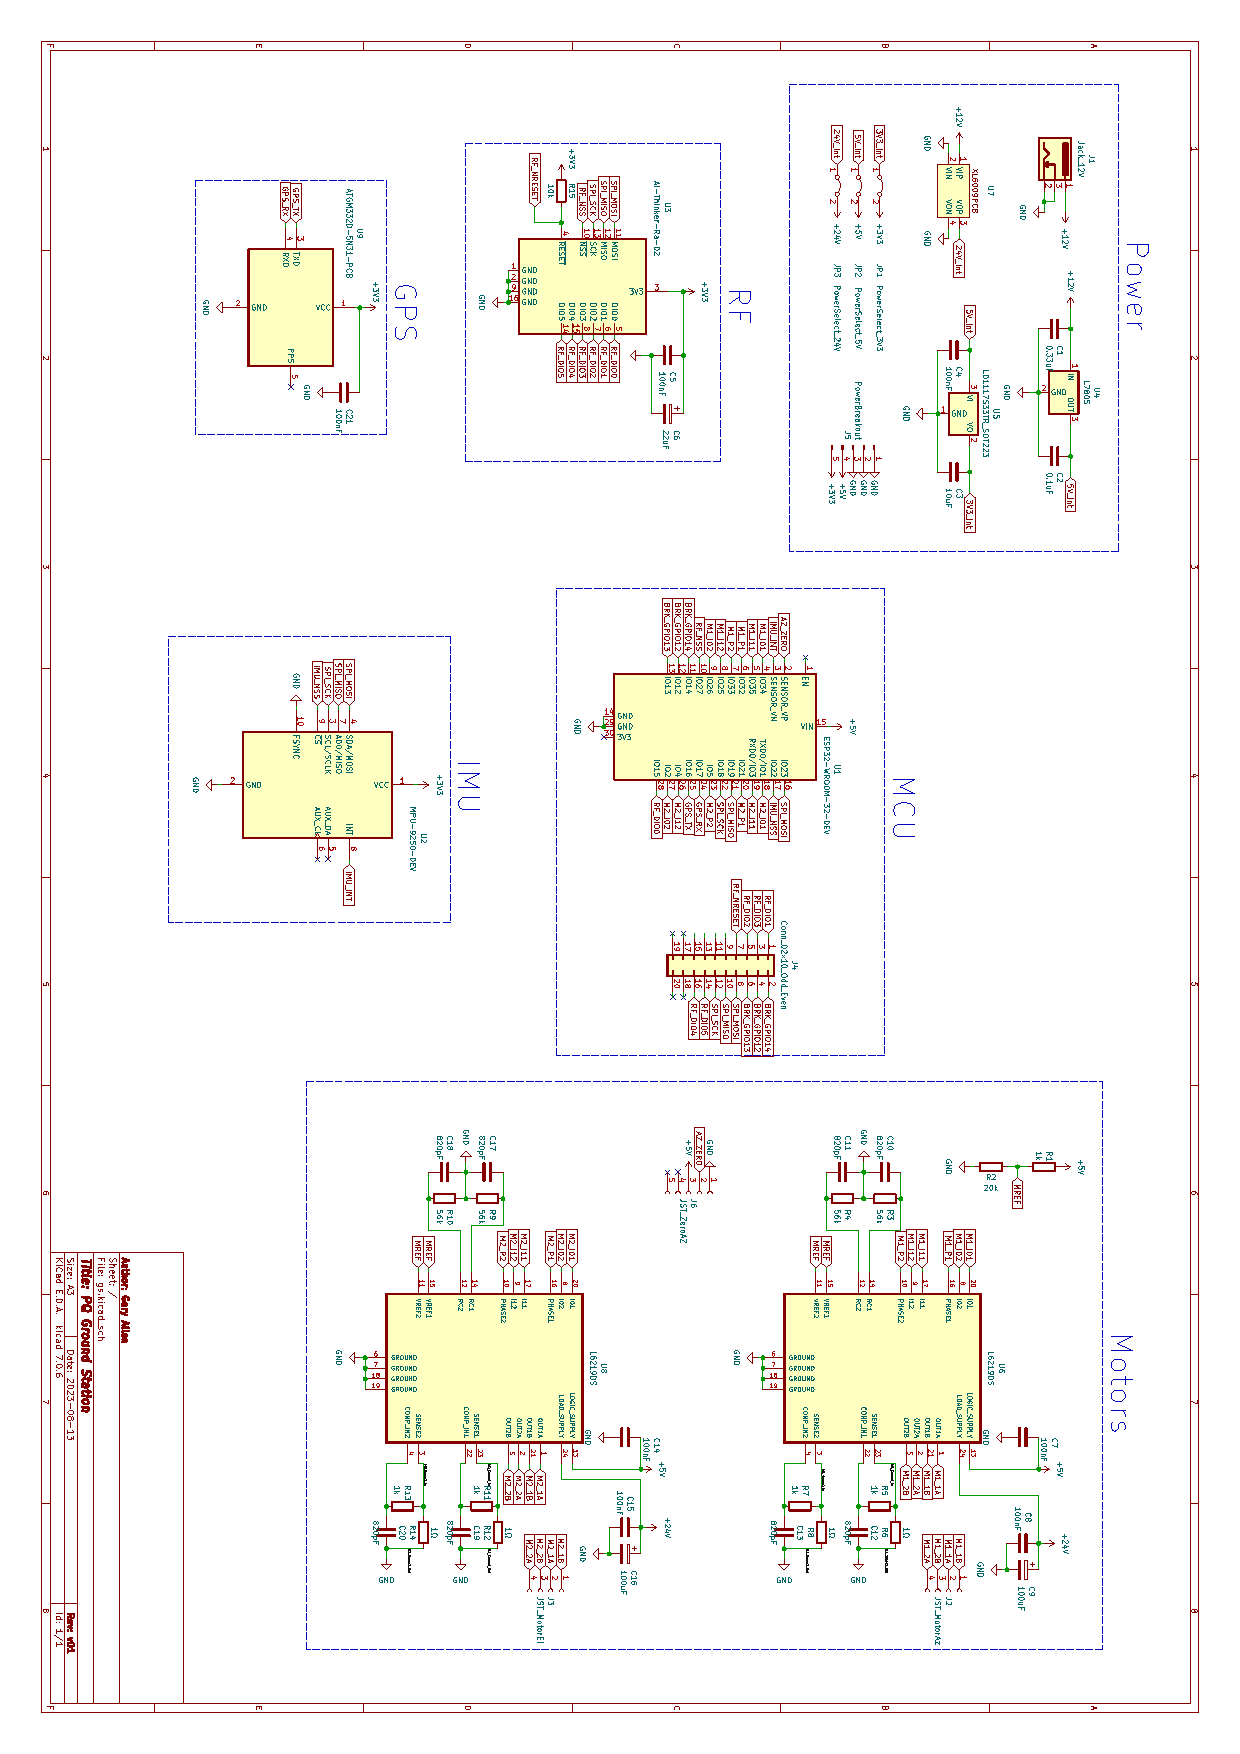
\includepdf[scale=0.85,pages=1,offset=0mm -10mm,pagecommand=\section{Ground Station Schematic}\label{sec:appendix_gs_schematics}]{docs/gs_schematic}
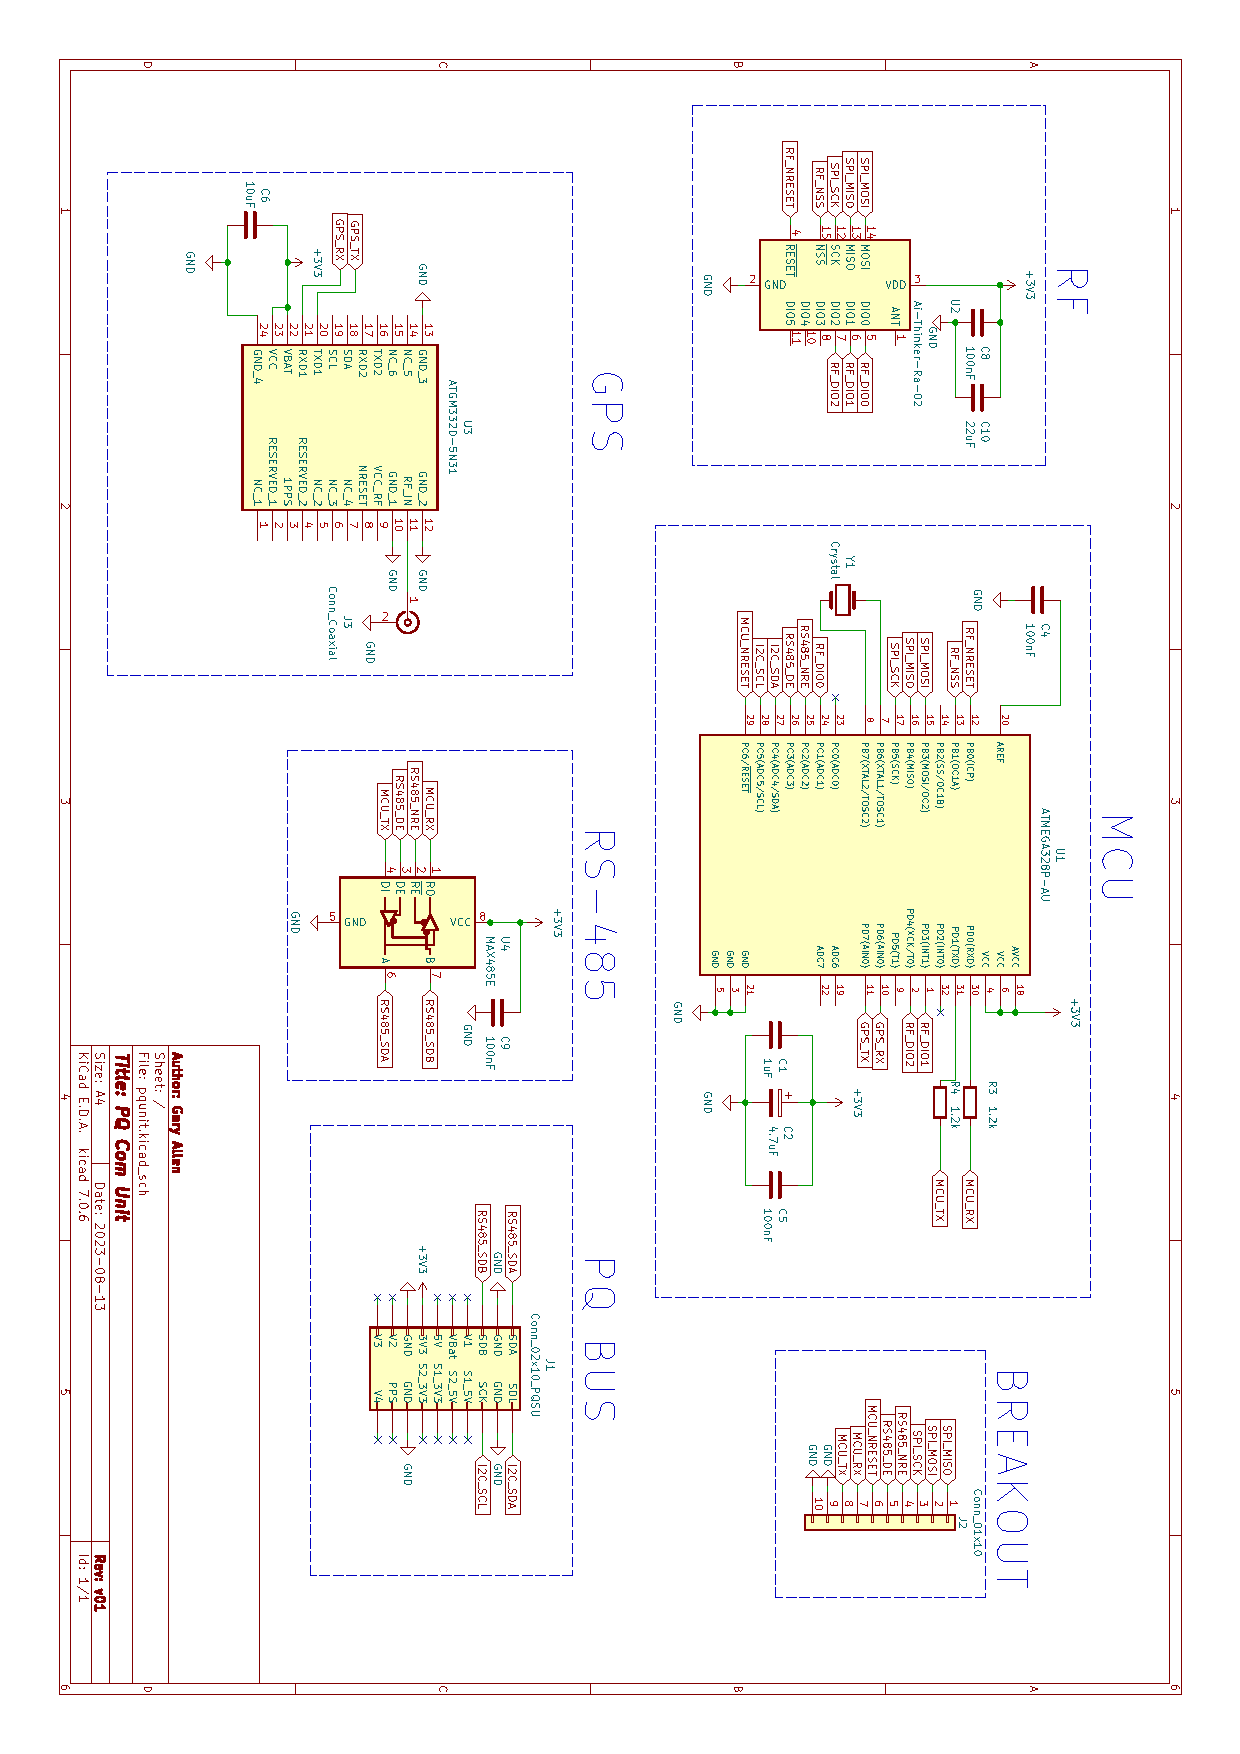
\includepdf[scale=0.85,pages=1,offset=0mm -10mm,pagecommand=\section{PocketQube Unit Schematic}\label{sec:appendix_pq_schematic}]{docs/pq_schematic}

\section{Ground Station PCB}\label{sec:appendix_gs_pcb_design}
\begin{figure}[!htb]
  \centering
  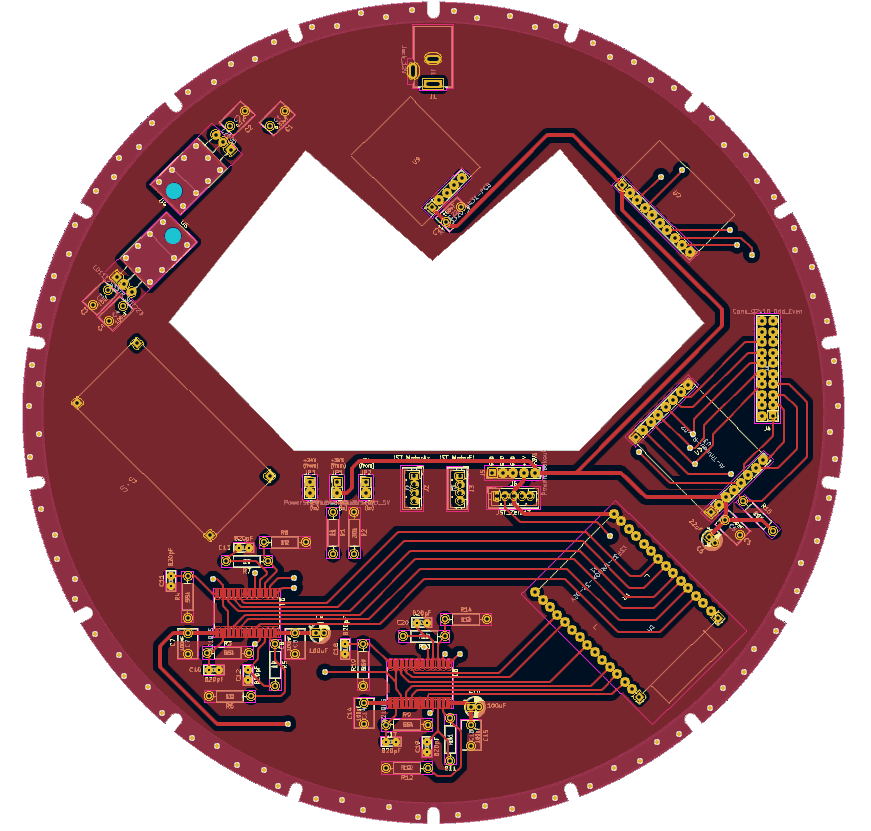
\includegraphics[width=0.95\textwidth]{gs_pcb_design_front}
  \caption{Ground Station PCB Design (front)}
  \label{fig:gs_pcb_design_front}
\end{figure}
\begin{figure}[!htb]
  \centering
  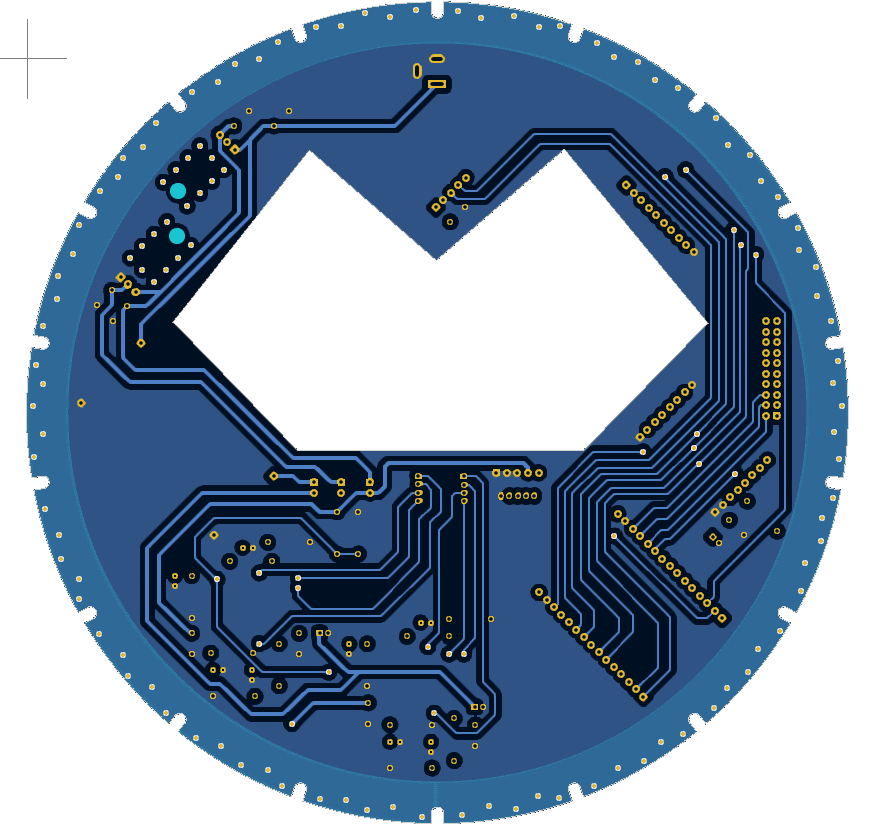
\includegraphics[width=0.95\textwidth]{gs_pcb_design_back}
  \caption{Ground Station PCB Design (back)}
  \label{fig:gs_pcb_design_back}
\end{figure}
\clearpage

\section{PCB Errata}\label{sec:appendix_pcb_errata}
Ground Station PCB:
\begin{itemize}
  \item The zero-sensor JST pin connections were incorrect.
  \item ESP Pins IO1 and IO3 should be left free for UART communication. Nets M2\_IO1 and M2\_I11 are therefore moved to pins IO14 and IO12 respectively.
  \item ESP Pins IO34 and IO35 are input-only. Nets M1\_I01 and M1\_I11 are therefore moved to pins IO0 and IO16 respectively. In this case, GPS\_TX is no longer used, and pin 0 on-board the ESP module on the board must be soldered to directly.
  \item The ESP development board's footprint was sized slightly to wide, and should be narrowed to avoid having to bend the pins.
\end{itemize}

\noindent PocketQube Unit PCB:
\begin{itemize}
  \item The loading capacitors on the crystal oscillator were incorrectly left out. The 8 MHz clock was therefore used, however the capacitors should be added in order for a 16 MHz clock to be used.
\end{itemize}

\section{Ground Station Antenna}
\begin{table}[!htb]
  \centering
  \renewcommand{\arraystretch}{1.2}
  \begin{tabular}{ |c|c| }
  \hline
  \textbf{Parameter}                  & \textbf{Value}    \\
  \hline
  Diameter (D)                        & 187.1 mm          \\ \hline
  Turn Spacing (S)                    & 88.2 mm           \\ \hline
  No. of Turns (n)                    & 4                 \\ \hline
  Ground plane diameter (G)           & $> \SI{350}{mm}$  \\ \hline
  Strip height (sh)                   & 19.4 mm          \\ \hline
  Strip width (sw)                    & 77.7 mm           \\ \hline
  Strip length (sl)                   & 132 mm           \\ \hline
  Cup height, if used (ch)            & 88.2 mm           \\ \hline
  \end{tabular}
  \caption{Helical Antenna Final Parameters}
  \label{tab:helicalParameters}
\end{table}

\newpage
\section{Software}
\begin{table}[!htb]
  \centering
  \caption{GPS Class}
  \renewcommand{\arraystretch}{1.2}
  \begin{tabular}{ |c|c| }
  \hline
  \textbf{Function}        & \textbf{Description}    \\
  \hline
    getLocation()              & Return latitude, longitude and altitude \\
    getTime()                  & Return seconds since epoch \\
  \hline
  \end{tabular}
  \label{tab:gpsUML}
\end{table}

\begin{table}[!htb]
  \centering
  \caption{Radio Class}
  \renewcommand{\arraystretch}{1.2}
  \begin{tabular}{ |c|c| }
  \hline
  \textbf{Function}        & \textbf{Description}    \\
  \hline
    startTransmit(message)              & Transmit data (non-blocking i.e. with callback) \\
    startReceive()                      & Start listening to receive data (non-blocking i.e. with callback) \\
    getRssi()                           & Get signal strength \\
    getSnr()                            & Get signal-to-noise ratio \\
  \hline
  \end{tabular}
  \label{tab:radioUML}
\end{table}

\begin{table}[!htb]
  \centering
  \caption{Link Class}
  \renewcommand{\arraystretch}{1.2}
  \begin{tabular}{ |c|c| }
  \hline
  \textbf{Function}        & \textbf{Description}    \\
  \hline
  setTelemetryCallback(fn)                    & Set the ``telemetry sent/received" function  \\
  setTelecommandCallback(fn)                  & Set the ``telecommand received" function (\textit{Responder} only) \\
  \hline
  \end{tabular}
  \label{tab:linkUML}
\end{table}

\begin{table}[!htb]
  \centering
  \caption{StepperMotor Class}
  \renewcommand{\arraystretch}{1.2}
  \begin{tabular}{ |c|c| }
  \hline
  \textbf{Function}        & \textbf{Description}    \\
  \hline
    stepForward(numSteps)         & Blocking and non-blocking options \\
    saveZeroPosition()            & Used for calibration \\
    getPosition()                 & Used for open-loop feedback \\
    setSpeed()                    & Sets the delay between steps \\
    setCurrentMultiplier()        & Set the amount of current \\
  \hline
  \end{tabular}
  \label{tab:stepperMotorUML}
\end{table}

\begin{table}[!htb]
  \centering
  \caption{Mount Class}
  \renewcommand{\arraystretch}{1.2}
  \begin{tabular}{ |c|c| }
  \hline
  \textbf{Function}        & \textbf{Description}    \\
  \hline
    calibrate()                         & Calbrate the mount \\
    setAzimuthalElevation(az, el)       & Set the azimuthal and elevation angles \\
    setBoresight(boresightVec)          & Set the boresight pointing vector \\
  \hline
  \end{tabular}
  \label{tab:mountUML}
\end{table}

\begin{table}[!htb]
  \centering
  \caption{GroundStation Class}
  \renewcommand{\arraystretch}{1.2}
  \begin{tabular}{ |c|c| }
  \hline
  \textbf{Function}             & \textbf{Description}    \\
  \hline
    calibrate()                 & Calibrate the entire GS \\
    addEstimatedLocation(loc)      & Add an estimated input GPS location for open-loop tracking \\
    addKnownLocation(loc)          & Add a known GPS location for closed-loop tracking \\
  \hline
  \end{tabular}
  \label{tab:groundStationUML}
\end{table}

\section{Mount Calibration}\label{sec:appendix_mount_calibration}

The calibration procedure of the mount is described below:
\begin{itemize}
  \item Measure the elevation angles of the mount at both extremes.
  \item Measure the offset angle between the zero-sensor and the desired magnetic north location.
  \item Lookup the magnetic declination near the area of interest.
  \item Include the previous three values statically in the software code.
  \item Rest the mount on the side with the larger elevation angle.
  \item Face the mount towards magnetic north.
  \item Run the mount's software calibration procedure, which rotates in azimuth until the zero sensor is found; then in elevation (open-loop) until the start elevation angle is reached; and finally faces north using the magnetic declination and offset angle.
\end{itemize}